\documentclass[12pt]{article}

\usepackage{hyperref}
\hypersetup{
	colorlinks,
	citecolor=blue,
	%filecolor=black,
	linkcolor=black,
	urlcolor=blue
}
\usepackage{float}
\usepackage[english]{babel}
\usepackage[square,numbers]{natbib}
\bibliographystyle{abbrvnat}
\usepackage{url}
\usepackage[utf8x]{inputenc}
\usepackage{amsmath}
\usepackage{graphicx}
\graphicspath{{images/}}
\usepackage{parskip}
\usepackage{fancyhdr}
\usepackage{vmargin}
\PassOptionsToPackage{hyphens}{url}\usepackage{hyperref}
\setmarginsrb{3 cm}{2.5 cm}{3 cm}{2.5 cm}{1 cm}{1.5 cm}{1 cm}{1.5 cm}
\usepackage[table]{xcolor}
\usepackage{todonotes}
\usepackage{menukeys}

\title{Project report}   % Title
\author{ Nikiforos Pittaras, M1422 \\ 
		 Chrysoula Themeli, M1423}                               % Authors
\date{\today}  % Date

\makeatletter
\let\thetitle\@title
\let\theauthor\@author
\let\thedate\@date
\makeatother

\pagestyle{fancy}
\fancyhf{}
%\rhead{\theauthor}
\lhead{\thetitle}
\cfoot{\thepage}

\begin{document}
	
	%%%%%%%%%%%%%%%%%%%%%%%%%%%%%%%%%%%%%%%%%%%%%%%%%%%%%%%%%%%%%%%%%%%%%%%%%%%%%%%%%%%%%%%%%
	
	\begin{titlepage}
		\centering
		\vspace*{0.5 cm}
		
\includegraphics[scale = 0.75]{ekpalogo.png}\\[1.0 cm]   % University Logo
		\textsc{\LARGE National and Kapodistrian University of Athens}\\[2.0 cm]   % University Name
		\textsc{\Large Department of Informatics and Telecommunications}\\[0.5 cm]               % Department
		\textsc{\large Large-Scale Data Analysis Techniques}\\[0.5 cm] % Course Name
		\rule{\linewidth}{0.2 mm} \\[0.4 cm]
		{ \huge \bfseries \thetitle}\\
		\rule{\linewidth}{0.2 mm} \\[1.5 cm]
		
		\begin{minipage}{0.4\textwidth}
			\begin{center} \large
				\theauthor
			\end{center}
		\end{minipage}~
		\begin{minipage}{0.4\textwidth}
		\end{minipage}\\[2 cm]
		
		{\large \thedate}\\[2 cm]
		
		\vfill
		
	\end{titlepage}
	
	%%%%%%%%%%%%%%%%%%%%%%%%%%%%%%%%%%%%%%%%%%%%%%%%%%%%%%%%%%%%%%%%%%%%%%%%%%%%%%%%%%%%%%%%%
	
	\tableofcontents
    \newpage
	\listoffigures
	\newpage
	
	%%%%%%%%%%%%%%%%%%%%%%%%%%%%%%%%%%%%%%%%%%%%%%%%%%%%%%%%%%%%%%%%%%%%%%%%%%%%%%%%%%%%%%%%%

	\section{Introduction}
    This is the report related to the Python project for the course "Large-Scale Data Analysis Techniques". In the below sections, the implemented logic will be explicitly analyzed. The project is divided in two parts: in the first part the goals are: to preprocess and clean the given data as well as to visualize five of the given trips in the train\_set file. In the second part, the tasks are: to find for all test trips the k nearest neighbors from the given train trips, to find the train trips with the longest similar sub-route for each test trip, to use 10-fold cross validation to the training data and classify them with three different methods (k-nearest neighbors, logistic regression and random forest), to choose one of the above classification methods and improve the result and finally to test the classifier on some given test data.
    
    In the \texttt{main.py} file, it is required to provide the path to the input folder (containing the training and test files) and the output folder where all results will be stored. Afterwards, an object containing all the necessary for the program options is created. This object includes options such as the given input and output directories, the train and the required test files, the number of cells in the grid to be constructed, the number of nearest neighbors etc. There are two ways in order to run this project, either add these folders in the edit configurations choice from the menu, or use the run.sh in order to provide these args. Finally, the dependencies are checked and the folders and files are prepared before starting to run the application.

  Some unclear points in the project instructions where dealt with respective
  variables and multiple implementations. These points where:
  \begin{itemize}
  \item Unique journey ids in subroutes (\texttt{unique\_jids} parameter,
    default true.)
    \item Consequtive common subsequences (\texttt{conseq\_lcss} parameter,
      default true.)
    \end{itemize}
    
	\section{Exercise 1}
	In this section, further details are provided related to the preprocessing and cleaning of the training data as well as to the trip's visualization. All files implementing the requirements of this part are in the file \texttt{question1.py}.
	
	\subsection{Data Preprocessing (question A)}
	The goal in this part is to preprocess the input training data and create a
  new file with 3 columns:
  \begin{itemize}
  \item  the trip\_id (a number incrementing by 1 for each trip)
  \item the journey\_id(excluding trips with null id)
  \item all points and timestamps in the format: [[timestamp1, longitude1,
    latitude1], [timestamp2, longitude2, latitude2],...].
  \end{itemize}
  The given csv file with the training data was transformed to a dataframe using
  the pandas library. Data with null journey ids are removed from the dataframe,
  therefore lines with NaN or "null" journey ids are discarded. All data is
  subsequently grouped by the vehicleID and the journeyPatternId. The final dataframe contains five columns, where the three last columns contain a list of timestamps, a list of longitudes and a list of latitudes respectively.
	
	To produce the required final format [timestamp, longitude, latitude], we
  iterate each row, producing a column with the appropriate list data. The total number of trips extracted to the trips.csv file is 6651.
  % the three lists are now concatenated in one column and therefore the other two are dropped from the dataframe. Then, the column vehicleID is replaced by the tripId column which is the index of this dataframe, starting from 0 and incrementing by 1. Finally, the column points, which now contains the list of lists with the timestamps and the points, is sorted based on the timestamp of each list item. The final result is exported in a file with the requested format.
	
	\subsection{Clean Data (question B)}
	We clean the given data based on two criteria:
  \begin{enumerate}
  \item the total trip distance should not be less than 2km
  \item the max distance between two successive points should not exceed 2km.
    \end{enumerate}
	
	The above logic is implemented in function \texttt{filter\_trips}. The two
  lists (\texttt{trips\_too\_small and trips\_too\_big}) will keep the trips
  discarded due to the aforementioned criteria. For each trip in the training
  dataset the total distance is calculated using the function
  \texttt{calculate\_total\_distance}, which uses the
  \texttt{calculate\_lonlat\_distance} function that returns the distance
  between two points using the haversine formula. Using these functions we
  compute the required distances and discard the trips that match the exclusion
  criteria.
	
	The resulting filtered trips are stored in the file \texttt{trips\_clean.csv}. The total number of filtered trips is 6020 (192 are deleted due to having total distance less than 2km while 439 are excluded due having to max distance between two points more than 2km).
	
	\subsection{Trip Visualization (question C)}
	This trip visualization task is implemented in the function
  \texttt{visualize\_trips} and the created output is stored in the output
  folder in the \texttt{gmplot} directory. The trips list is shuffled in order
  to show random items, the first 5 of which are fetched for
  visualization. For each trip, we generate a tuple of longitudes and latitudes
  with the function \texttt{utils.idx\_to\_lonlat} which we pass on to the
  plotting function \texttt{utils.write\_group\_gml}. There, the longitude and
  latitude means are calculated as a visualization centroid for the produced map, and the gmplot
  library is used so as to visualize the respective point sequence. See the
  following figure for a visualization example. 
	
	\begin{figure} [H]
		\begin{center}
			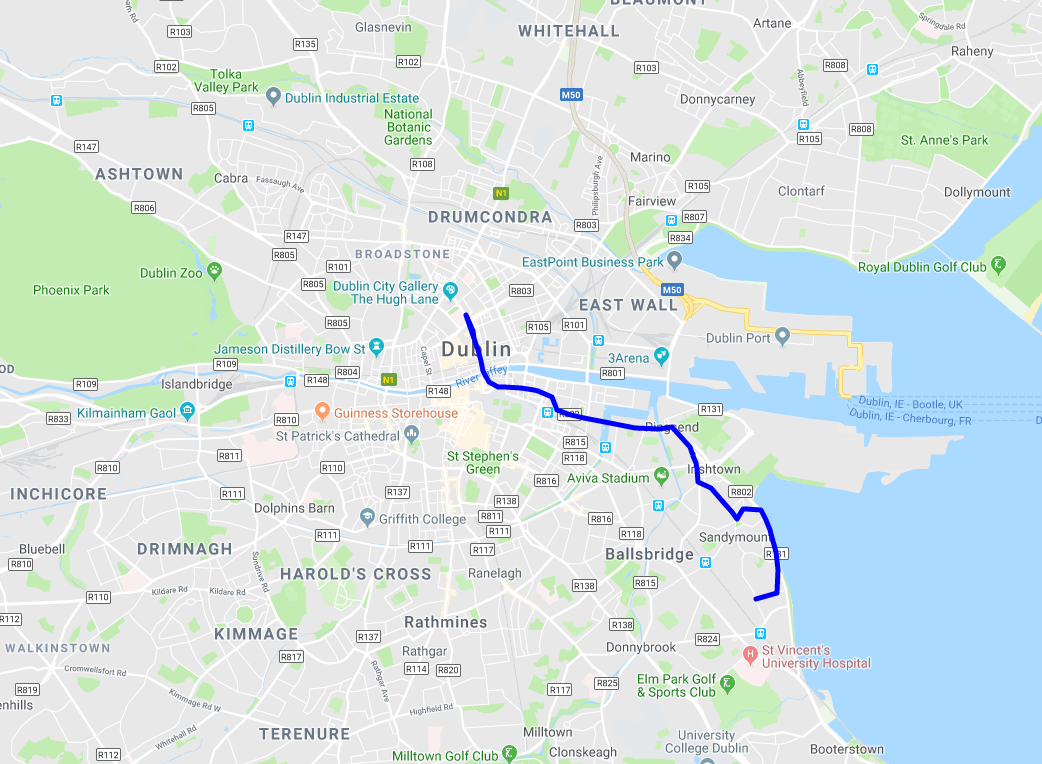
\includegraphics [scale = 0.55] {questionC1.png}
			\caption{First trip visualization.}
		\end{center}
    \label{gmlplot_example}
	\end{figure}

	\begin{figure} [H]
		\begin{center}
			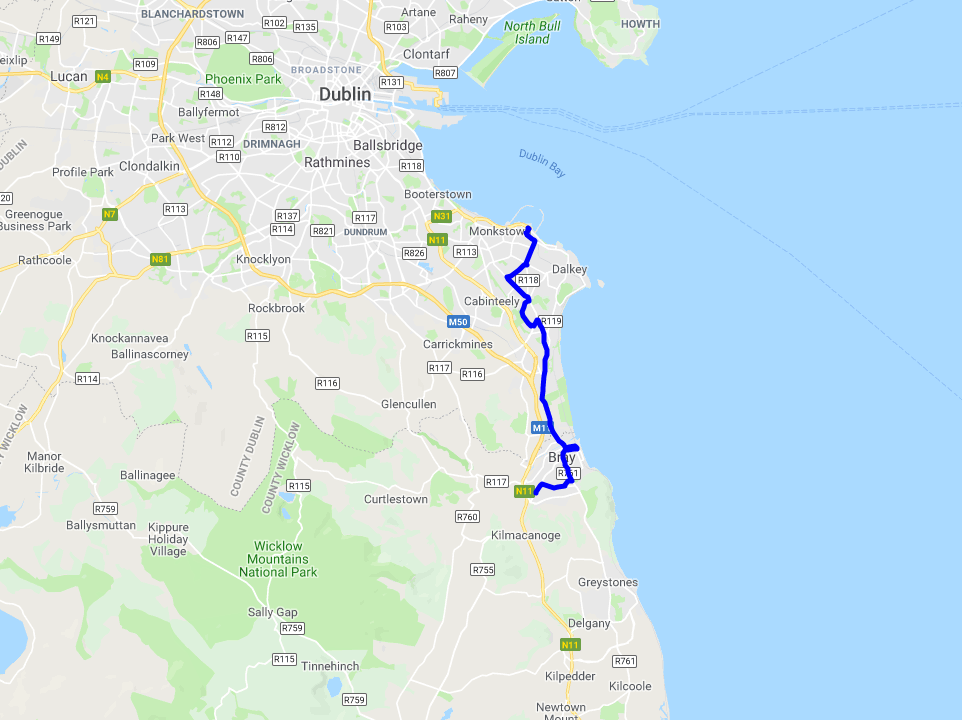
\includegraphics [scale = 0.60] {questionC2.png}
			\caption{Second trip visualization.}
		\end{center}
		\label{gmlplot_example}
	\end{figure}

	\begin{figure} [H]
		\begin{center}
			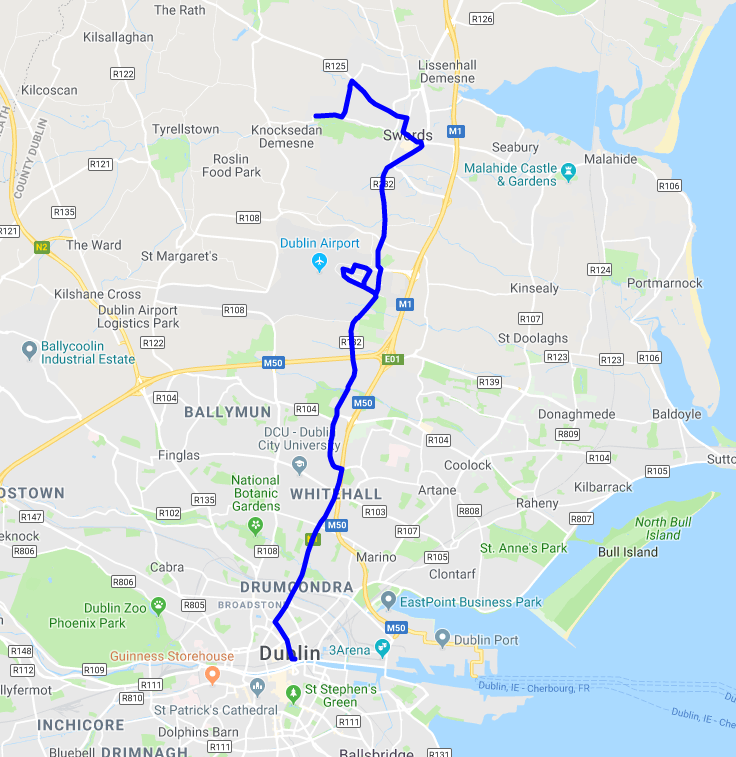
\includegraphics [scale = 0.75] {questionC3.png}
			\caption{Third trip visualization.}
		\end{center}
		\label{gmlplot_example}
	\end{figure}

	\begin{figure} [H]
		\begin{center}
			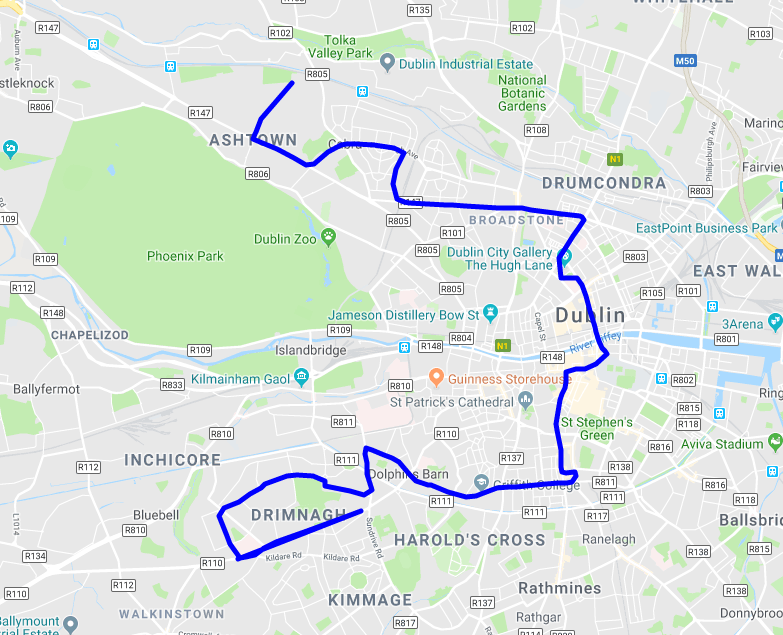
\includegraphics [scale = 0.75] {questionC4.png}
			\caption{Third trip visualization.}
		\end{center}
		\label{gmlplot_example}
	\end{figure}

	\begin{figure} [H]
		\begin{center}
			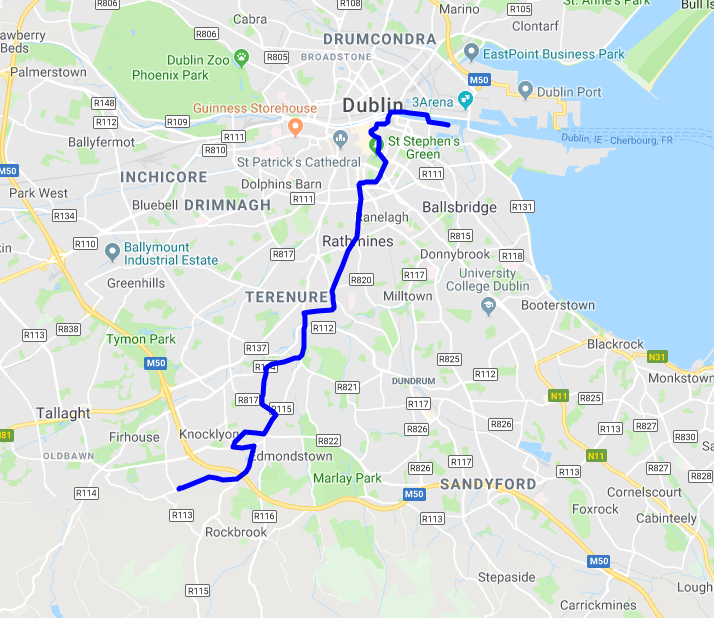
\includegraphics [scale = 0.75] {questionC5.png}
			\caption{Third trip visualization.}
		\end{center}
		\label{gmlplot_example}
	\end{figure}
	
	\section{Exercise 2}
	This exercise is implemented in the file question2.py and some functions implementing the logic for this question are in the files: \texttt{NearestNeighbors.py, NearestSubroutes.py, MapInGridView, JourneyClassification.py}.
	
	\subsection{Nearest Neighbors (question A1)}
	For this part, a test file is given (test\_set\_a1.csv, included in the input
  folder) containing additional test trip data. For each test trip, the k
  nearest neighbors are extracted (in this exercise k=5) and an image file is
  produced, showing all six trips (the test trip and its 5 neighbour trips from the training file) on six different maps. Under each map, the test or neighbor index, the journey\_id, the dynamic time warping and the time needed to process the neighbors of this test trip in millisecond.
	
	In the function \texttt{question\_a1}, two dataframes are created for both the
  test and the training trips. For each test trip, \texttt{calculate\_nns} from
  the file NearestNeighbors.py is called in order to get the nearest neighbors
  with respect to all training trips, calculating also the time needed for this calculation.
	
	In \texttt{calculate\_nns}, we explored parallelization options to compute the neighbours,
  due to the computational intensivenes of the task.
  \begin{enumerate}
  \item using multiple processes (\texttt{run\_with\_processes} function) with the
    \texttt{multiprocessing} module, where an async task is executed for each process.
  \item multiple threads (\texttt{run\_with\_threads} function) with the \texttt{threading} module, where the task is
    broken to multiple threads with separate result containers.
  \item standard serial execution, where each training datum is examined iteratively.
  \end{enumerate}
  This parallelization type and parameter (i.e. number of processes or threads) is contained in tie \texttt{paropts} variable in main.
	
	In the function \texttt{calculate\_dists}, the 3rd column of the dataframe is
  provided and
  In the function, each training trip's time series data is transformed to a
  list of (longitude, latitude) tuples, which is passed to the \texttt{calculate\_dynamic\_time\_warping}
  function to calculate the DTW distance. The latter is computed using the
  harvesine distance calculation function and the DTW wikipedia lemma. The
  resulting list contains the training instance information along with its distance to
  the test trip. Sorting the list to increasing distance and keeping its k first
  elements provides the k nearest neighbours.
	
	
  To visualize the neighbours, the \texttt{visualize\_nns}
  function is used, where three lists are created:
  \begin{enumerate}
    \item a list with all the route points (longitudes and latitudes) of the
      test trip and its neighbours
    \item a list with the journey labels and the nn computation data
      \item a list with the colors with which to draw (all blue in this
        question).
      \end{enumerate}
      All this data is provided to the
      \texttt{utils.visualize\_point\_sequences} function. This function is
      supplied with point sequences with corresponding color sequences, and
      produces colored gml plot maps with the \texttt{write\_group\_gml}
      function. Each html output map is converted to a png image using a conversion tool in the \texttt{html\_to\_png} function, in
order to automate image creation from the generated maps (the tool is the
\texttt{rasterize.js} utility from the \texttt{phantomjs} module).
However we found the gml plot zoom difficult to automatically configure correctly so that
all points are visible, and thus the images in the report were fetched with a printscreen.
The converted images are used to create 6 subplots (1 test trip + k=5 nearest
neighbours). All plotting is done with the pylab package.

	Below we present the results from this question in the requested format:
	
	\begin{figure} [H]
		\begin{center}
			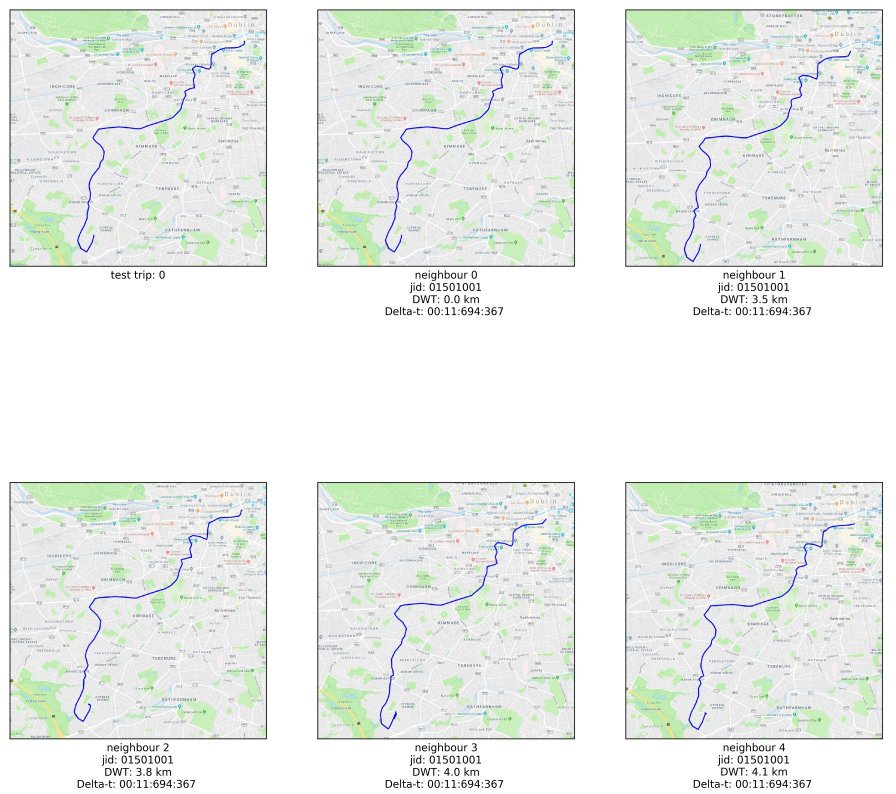
\includegraphics [scale = 0.60] {nn1.png}
			\caption{Nearest neighbours for the first test trip}
		\end{center}
	\end{figure} 

	\begin{figure} [H]
		\begin{center}
			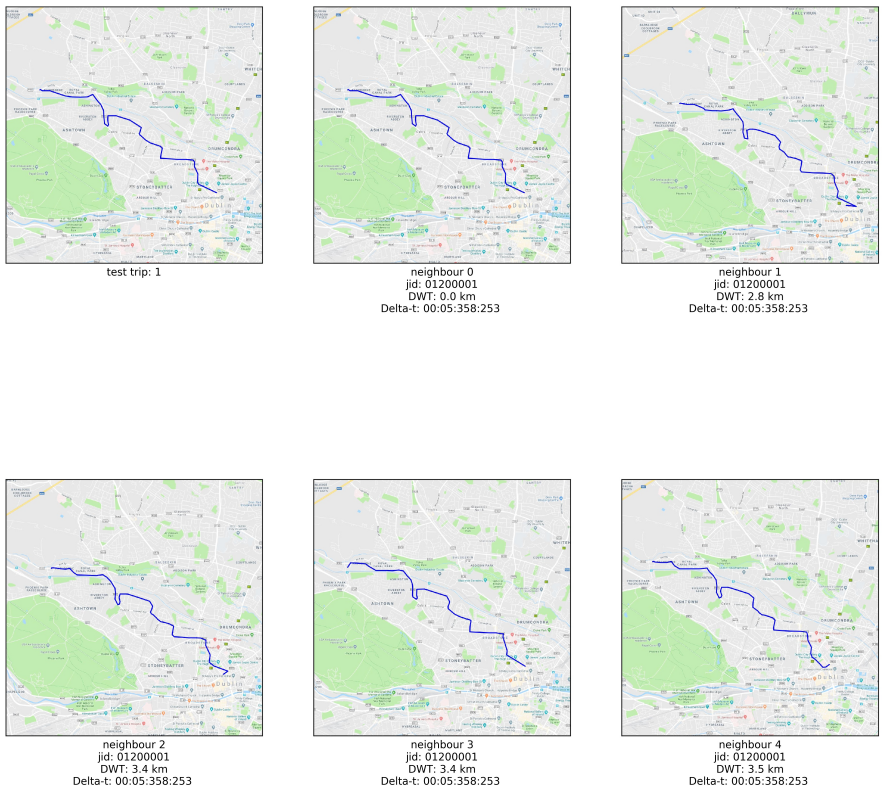
\includegraphics [scale = 0.60] {nn2.png}
			\caption{Nearest neighbours for the second test trip}
		\end{center}
	\end{figure}

	\begin{figure} [H]
		\begin{center}
			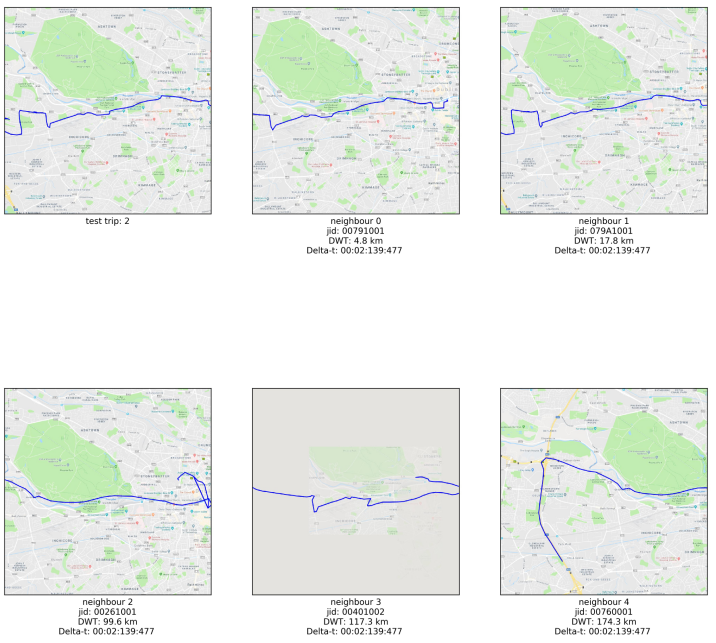
\includegraphics [scale = 0.60] {nn3.png}
			\caption{Nearest neighbours for the third test trip}
		\end{center}
	\end{figure} 

	\begin{figure} [H]
		\begin{center}
			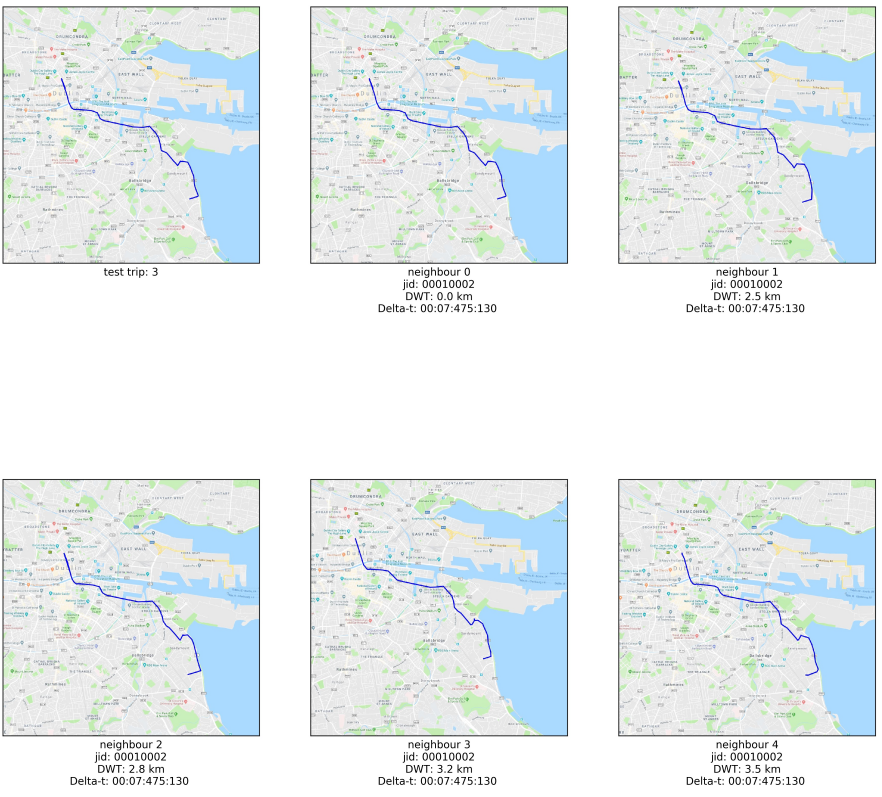
\includegraphics [scale = 0.60] {nn4.png}
			\caption{Nearest neighbours for the fourth test trip}
		\end{center}
	\end{figure} 

	\begin{figure} [H]
		\begin{center}
			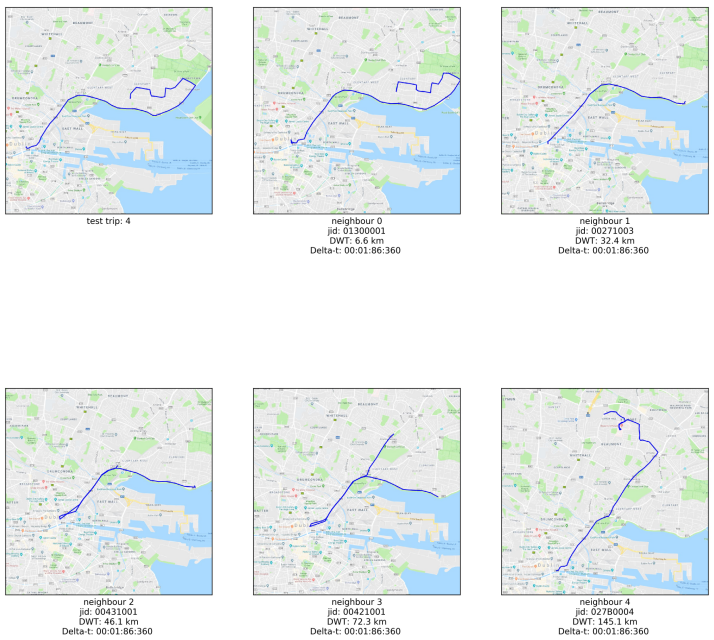
\includegraphics [scale = 0.60] {nn5.png}
			\caption{Nearest neighbours for the fifth test trip}
		\end{center}
	\end{figure} 

	In \ref{nnresults}, we show the total results for the Nearest Neighbors.
	
	\begin{table}[H]
		\centering
		\begin{tabular}{|c|c|c|c|c|c|c|c|c|c|c|c|}
			\hline
			\textbf{}  & \textbf{Time} & \textbf{id1} & \textbf{d1} & \textbf{id2} & \textbf{d2} & \textbf{id3} & \textbf{d3} & \textbf{id4} & \textbf{d4} & \textbf{id5} & \textbf{d5} \\ \hline
			\textbf{1} & 11:694:365    & 4139          & 0.0           & 1756         & 3.5           & 584         & 3.8           & 3119          & 4.0           & 3428         & 4.1           \\ \hline
			\textbf{2} & 05:358:252     & 1554          & 0.0           & 6461          & 2.8          & 1985          & 3.4          & 611         & 3.4         & 1434         & 3.5         \\ \hline
			\textbf{3} & 12:732:353    & 3317         & 0.0           & 1939          & 4.7           & 3200          & 4.8           & 5374          & 4.8           & 1508          & 4.8          \\ \hline
			\textbf{4} & 07:475:129     & 603         & 0.0           & 559          & 2.5           & 951         & 2.8           & 1118          & 3.2          & 684          & 3.5          \\ \hline
			\textbf{5} & 07:444:862     & 1497          & 0.0           & 1688         & 4.3          & 927         & 4.5          & 2578         & 4.6          & 6252         & 4.7         \\ \hline
		\end{tabular}
	\caption{Nearest Neighbors results}
	\label{nnresults}
	\end{table}
	
	\subsection{Nearest Sub-routes (question A2)}
	Following the same logic as above, in the function \texttt{question\_a2} we
  compute the nearest subroutes of each test trip with the following key
  differences:
  \begin{itemize}
    \item Instead of DTW, we use the LCSS algorithm in the \texttt{calc\_lcss}
      method, using the harvesine formula for pointwise distance as before. Give
      a test and train point sequence, the LCSS function returns a list of all
      common subsequence points and indexes of the two sequence inputs. The
      parameter \texttt{unique\_jids} controls wether more than one subsequence
      is allowed per training trip (default false). Based on the exercise
      requirements, two points are considered as equals if their distance is less than 200 metres.

      \item The collection of longest subsequences is updated on-line in the
        \\ \texttt{update\_current\_maxsubseq} function. Each new subsequences list
        from a training trip is sorted length-wise, and the current max k
        subsequences list is updated accordingly (i.e. if there is enough space
        or if thew new entries are longer than existing ones). Special care is
        taken to keep unique journey ids, if the \texttt{unique\_jids} is activated.
      \end{itemize}
	
	Finally, a similar data preparation is followed as with the nearest neighbour
  case to visualize the data. For each training trip, the points belonging to
  the subroute are colored red, while the others are plotted in blue, by storing
  corresponding point lists and colors to lists. The required metadata are
  supplied as labels to the \texttt{utils.visualize\_point\_sequences} function,
  as before.
	
  Below, we present the nearest subroutes for each given test trip:
	
	\begin{figure} [H]
		\begin{center}
			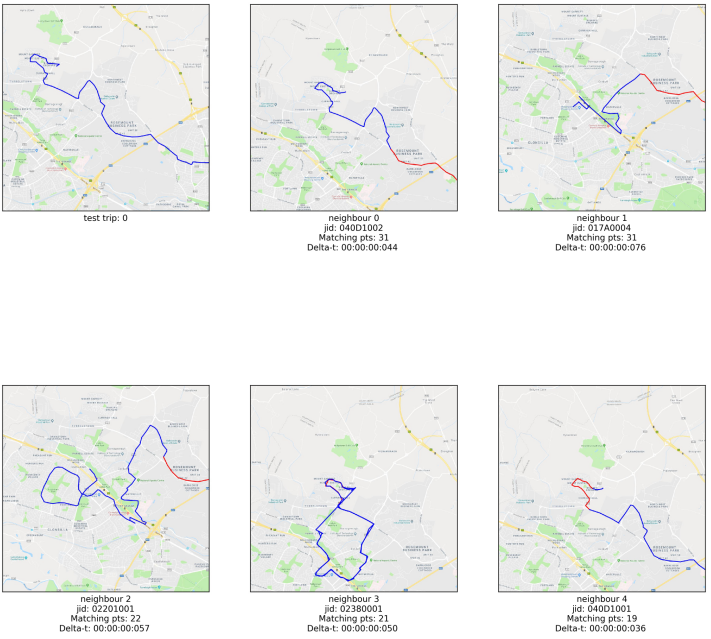
\includegraphics [scale = 0.80] {subroutes1.png}
			\caption{Nearest subroutes for the first test trip}
		\end{center}
	\end{figure} 
	
	\begin{figure} [H]
		\begin{center}
			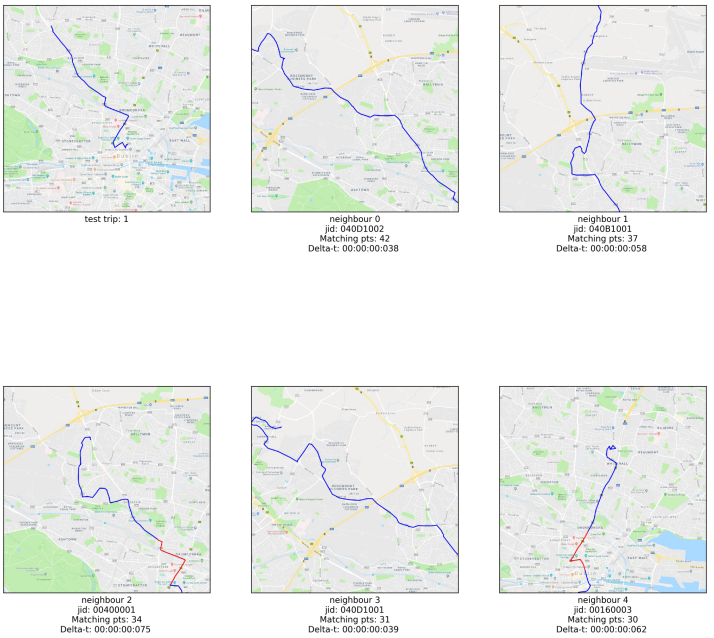
\includegraphics [scale = 0.80] {subroutes2.png}
			\caption{Nearest subroutes for the second test trip}
		\end{center}
	\end{figure}
	
	\begin{figure} [H]
		\begin{center}
			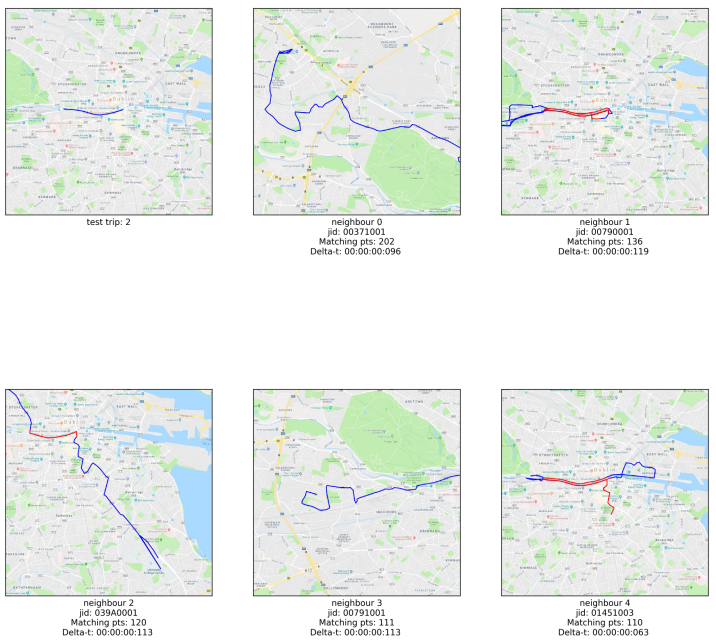
\includegraphics [scale = 0.80] {subroutes3.png}
			\caption{Nearest subroutes for the third test trip}
		\end{center}
	\end{figure} 
	
	\begin{figure} [H]
		\begin{center}
			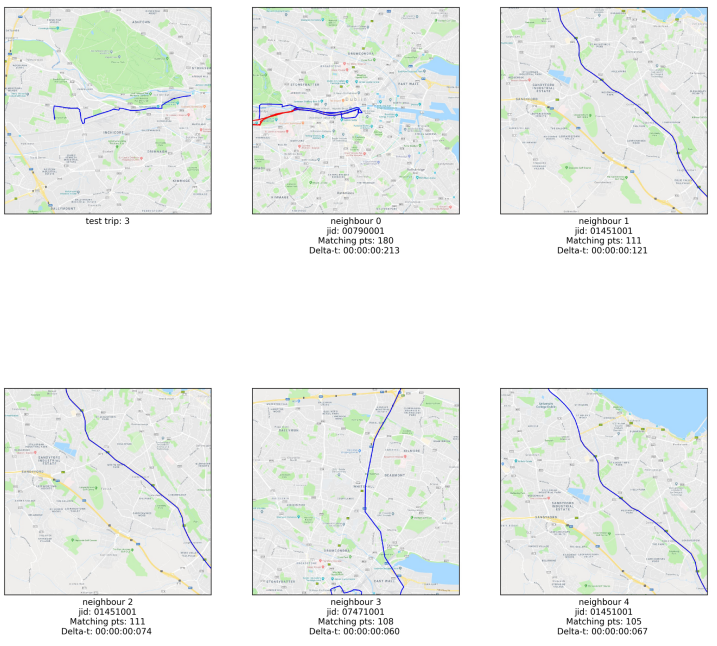
\includegraphics [scale = 0.80] {subroutes4.png}
			\caption{Nearest subroutes for the fourth test trip}
		\end{center}
	\end{figure} 
	
	\begin{figure} [H]
		\begin{center}
			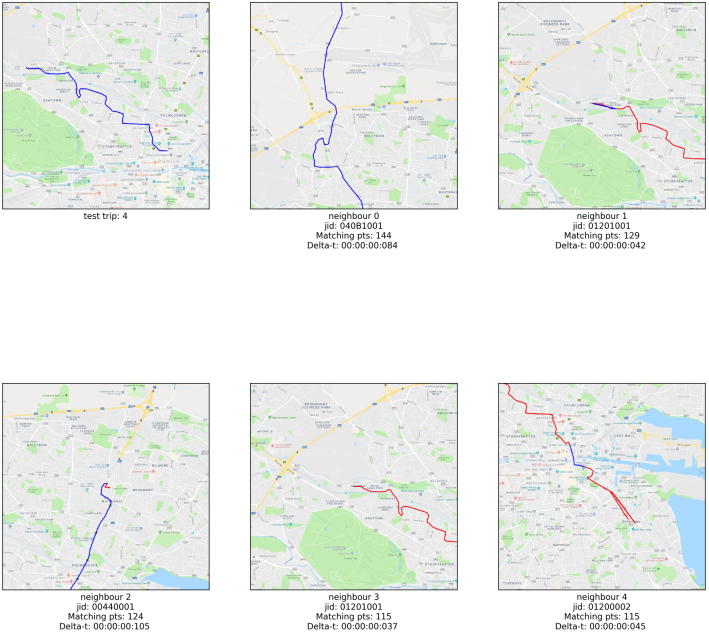
\includegraphics [scale = 0.80] {subroutes5.png}
			\caption{Nearest subroutes for the fifth test trip}
		\end{center}
	\end{figure}

	As in the Nearest Neighbours case, we have also included the html files in the gmplot folder. in \ref{subres} we show the total results for Nearest Subroutes.
	
	\begin{table}[H]
		\centering
		\begin{tabular}{|c|c|c|c|c|c|c|c|c|c|c|c|}
			\hline
			\textbf{}  & \textbf{Time} & \textbf{id1} & \textbf{pts1} & \textbf{id2} & \textbf{pts2} & \textbf{id3} & \textbf{pts3} & \textbf{id4} & \textbf{pts4} & \textbf{id5} & \textbf{pts5} \\ \hline
			\textbf{1} & 05:346:265     & 211          & 31            & 728          & 31            & 3590         & 22            & 4985          & 21            & 843          & 19            \\ \hline
			\textbf{2} & 01:63:755     & 2620         & 42            & 510          & 37            & 1093         & 34            & 426          & 31            & 363          & 30            \\ \hline
			\textbf{3} & 00:32:319     & 200          & 40            & 1885         & 40            & 2763         & 40            & 142          & 39            & 135          & 35            \\ \hline
			\textbf{4} & 00:46:297     & 566          & 32            & 1269         & 21            & 227          & 20            & 2561         & 17            & 252          & 15            \\ \hline
			\textbf{5} & 00:57:303     & 940          & 33            & 1932         & 22            & 1384         & 21            & 1606         & 21            & 1822         & 20            \\ \hline
		\end{tabular}
	\caption{Nearest subroutes results}
	\label{subres}
	\end{table}
	
	\subsection{Feature extraction (question B)}
	The purpose of this task was to extract features for classification from the
  training dataset. In short, a quantization grid should be created and the points of each trip trace should be replaced by a specific square of the grid. The output file where the exported features are stored is \texttt{tripFeatures.csv}.
	
The grid is assumed to be rectangular, with dimensions specified in the options
dictionary. In order to be able to draw the grid, we find the min and max
longitudes and latitudes (function: \texttt{find\_min\_max\_latlong}, file:
\texttt{MapInGridView.py}). The next function called is the
\texttt{create\_grid}, parameterized with the discovered bounds and the grid
dimensions. The next step is to create the lines of the rows and the columns and
then to provide a name for each cell. The training points and grid structure is
visualized with the \texttt{visualize\_grid} function, and illustrated in the
figures below.
	

	\begin{figure} [H]
		\begin{center}
			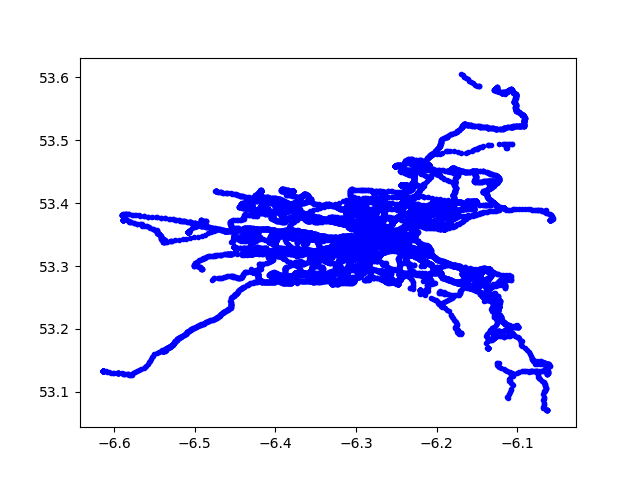
\includegraphics [scale = 0.70] {data_minmax_grid_extent.png}
			\caption{Training data for grid creation.}
		\end{center}
	\end{figure} 
	\begin{figure} [H]
		\begin{center}
			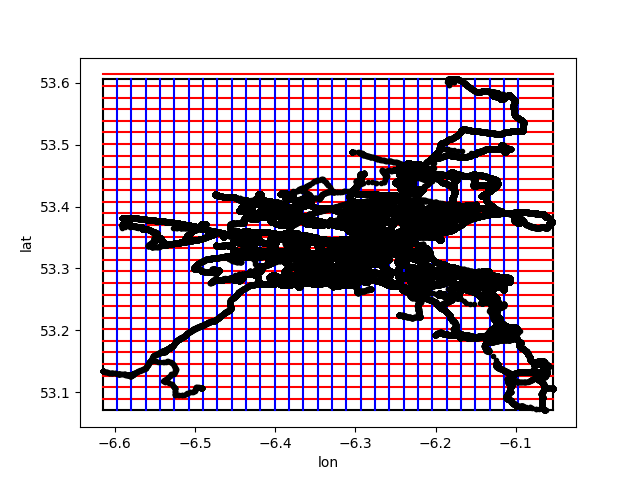
\includegraphics [scale = 0.70] {grid.png}
			\caption{Example rectangular quantization grid of 5 cells, resulting in 4
        row and column lines.}
		\end{center}
	\end{figure} 



  Feature construction uses the bag-of-words technique with the \texttt{map\_to\_features\_bow} function. A histogram vector is
  initialized to zeros for each trip, and each coordinate point in the trip is 
  mapped to a grid cell as a function of the grid rows, grid columns and the
  point's coordinates (funtion \texttt{find\_cell\_index}). This assignment increases the accumulation on that
  cell in the histogram vector. The resulting feature fectors are saved in a csv file.

	\subsection{Classification (question C)}
 All functions used in this question are in the file \texttt{JourneyClassification.py}. 
	In the method \texttt{question\_c}, a new dataframe is created from the
  features file, containing the quantized features.
  Data is prepared for classification in the method
  \texttt{preprocess\_train\_data}. There, data is shuffled and the target
  journey ids are uniquely mapped to integers to serve as target classes.

  The \texttt{train} function uses the numpy scikit-learn libraries to perform training.
  Data are converted to numpy arrays, partitioned to K=10 cross-validation folds
  and training is performed for each fold using the appropriate scikit-learn
  implementations for the Logistic Regression, Random Forests K-Nearest Neighbours (K=5)
  classifiers and the cross-validation itself. In summary, each classifier is
  implemented as an object, is trained and evaluated with the \texttt{fit} and
  \texttt{predict} functions respectively. Prediction produces the predicted
  classes in all classifiers but the Logistic Regression, which outputs class
  probabilities - there, the predicted class index is extracted by considering
  the argmax of the output. Training and validation accuracy
  is collected per fold and classifier with the \texttt{accuracy\_score} function
  of scikit-learn, both illustrated in a barchart, constructed using
  pylab and matplotlib. The mean accuracies accross folds is returned and printed.

  For beating the benchmark we have selected the Logistic Regression classifier,
  and attempted to improve its performance by the following techniques:
  \begin{itemize}
    \item Feature normalization, where we reduce the variance in the data by
      applying feature normalization techniques, using the $L_1, L_2$ and $max$ norms.
      \item Feature scaling, where the features are scaled to zero mean and unit variance.
    \item Varying the regularization term ($C$) in the Logistic Regression hyperplane
      to attempt to find a better fit in the data. We tested values from $0.2$ to $2$.
     \item Replace the bag-of-words feature with the VLAD (Vector of Locally
       Aggregated Descriptors) feature. In VLAD,
       instead of considering frequency histograms, we accumulate difference
       from the representative elements in the quantization vector. For example,
       if a point $p$ is assigned to cell $c_n$, in bag-of-words the $n$-th
       coordinate in the quantization vector is incremented by $1$. In VLAD, the
       increment equals $d(p,c_n)$, where $d(\cdot,\cdot)$ is a distance function.
       We used the cell centroid as the cell representative point and the
       harvesine distance. 
     
  \end{itemize}
  Results for all methods are in the table below.
 
 \begin{table}[H]
 	\centering
 	\begin{tabular}{|c|c|c|}
 		\hline
 		\textbf{Strategy}            & \textbf{Train Accuracy} & \textbf{Validation Accuracy} \\ \hline
 		\textbf{KNN}                 & 0.446                   & 0.221                        \\ \hline
 		\textbf{Logistic Regression} & 0.269                   & 0.170                        \\ \hline
 		\textbf{Random Forest}       & 0.969                   & 0.281                        \\ \hline
 	\end{tabular}
 \caption{Classification using KNN, logreg and random forest}
 \label{class}
 \end{table}

\begin{table}[H]
	\centering
	\begin{tabular}{|l|c|c|}
		\hline
		strategy & validaton accuracy & change  \\ \hline
		norm\_l2 &  0.063  &  -62.84\%  \\ \hline
		norm\_l1 &  0.048  &  -71.56\%  \\ \hline
		norm\_max &  0.072  &  -57.34\%  \\ \hline
		scaling &  0.131  &  -22.94\%  \\ \hline
		C\_0.200 &  0.15  &  -11.93\%  \\ \hline
		C\_0.500 &  0.157  &  -7.80\%  \\ \hline
		C\_1.500 &  0.175  &  2.75\%  \\ \hline
		C\_2.000 &  0.178  &  5.05\%  \\ \hline
		vlad &  0.003  &  -97.71\%  \\ \hline
		
	\end{tabular}
	\label{impr}
	\caption{Classification improvements using logistic regression}
\end{table}

	\subsection{Test improved classifier}
	
  We tested the improved classifier in the test data. The results are attached
  in the specified format to the file \texttt{testSet\_journeyPatternIDs.csv}.
	
	\newpage
	\addcontentsline{toc}{section}{References}
	\begin{thebibliography}{30}
		\bibitem{knn}SciKit Learn: Nearest Neighbors \\
		 \url{http://scikit-learn.org/stable/modules/neighbors.html}
		 \bibitem{logreg} SciKit Learn: Logistic Regression \\
		 \url{http://scikit-learn.org/stable/modules/linear_model.html#logistic-regression}
		 \bibitem{ranfor} SciKit Learn: Random Forest \\
		 \url{http://scikit-learn.org/stable/modules/generated/sklearn.ensemble.RandomForestClassifier.html#sklearn.ensemble.RandomForestClassifier}
		 \bibitem{accuracy} SciKit Learn: Accuracy \\
		 \url{http://scikit-learn.org/stable/modules/generated/sklearn.metrics.accuracy_score.html#sklearn.metrics.accuracy_score}
		 \bibitem{knn2}A Complete Guide to K-Nearest-Neighbors with Applications in Python and R \\
		 \url{https://kevinzakka.github.io/2016/07/13/k-nearest-neighbor/}
		 \bibitem{dwt} Dynamic time warping \\
		 \url{https://en.wikipedia.org/wiki/Dynamic_time_warping}
		 \bibitem{lcss} Longest common subsequence problem \\
		 \url{https://en.wikipedia.org/wiki/Longest_common_subsequence_problem}
		 \bibitem{report} SciKit Learn: Classification report \\
		 \url{http://scikit-learn.org/stable/modules/generated/sklearn.metrics.classification_report.html}
		 \bibitem{threads} ThreadPool \\
		 \url{https://stackoverflow.com/questions/8533318/multiprocessing-pool-when-to-use-apply-apply-async-or-map}
    \end{thebibliography}
	
\end{document}
